% Proposed architecture (not implemented yet), landscape A4, same style as pipeline_diagrams_landscape.tex.
% (1) inference pipeline, (2) SB-LN construction and parameter budget, (3) training workflow with GBRA,
% (4) novelty summary.  Rank r and head form are fixed by M10a / M10b before implementation (M11).
% Compile with:  tectonic proposed_architecture_landscape.tex
\documentclass[11pt]{article}
\usepackage[a4paper,landscape,margin=14mm]{geometry}
\usepackage{lmodern}
\usepackage{amsmath,amssymb}
\usepackage{xcolor}
\usepackage{array,booktabs}
\usepackage{tikz}
\usetikzlibrary{arrows.meta,positioning,fit,backgrounds,calc}
\pagestyle{empty}
\setlength{\parindent}{0pt}
\newcolumntype{L}[1]{>{\raggedright\arraybackslash}p{#1}}

\definecolor{box}{HTML}{EEF2F7}
\definecolor{trn}{HTML}{FCE9C8}
\definecolor{frz}{HTML}{DCE6F2}
\definecolor{prv}{HTML}{E3F1DF}

\tikzset{
  blk/.style={draw,rounded corners=3pt,fill=box,align=center,font=\normalsize,minimum height=19mm,text width=46mm,line width=0.8pt},
  frz/.style={blk,fill=frz},
  trn/.style={blk,fill=trn},
  prv/.style={blk,fill=prv},
  lab/.style={font=\footnotesize,text=black!80,inner sep=1.5pt},
  ar/.style={-{Latex[length=3mm]},line width=1.1pt}}

\newcommand{\sg}{\operatorname{sg}}

\begin{document}

% ---------------------------------------------------------------------
% PAGE 1: proposed inference pipeline
% ---------------------------------------------------------------------
\begin{center}
{\Large\bfseries Proposed Architecture --- Inference Pipeline (SB-LN + Real-Anchored Cosine Head)}\\[2pt]
{\small Proposed, not implemented. Orange = trained (17,186 numbers at \(r=8\)); blue = frozen; grey = fixed computation or stored buffer.}
\end{center}
\vspace{4mm}

\begin{center}
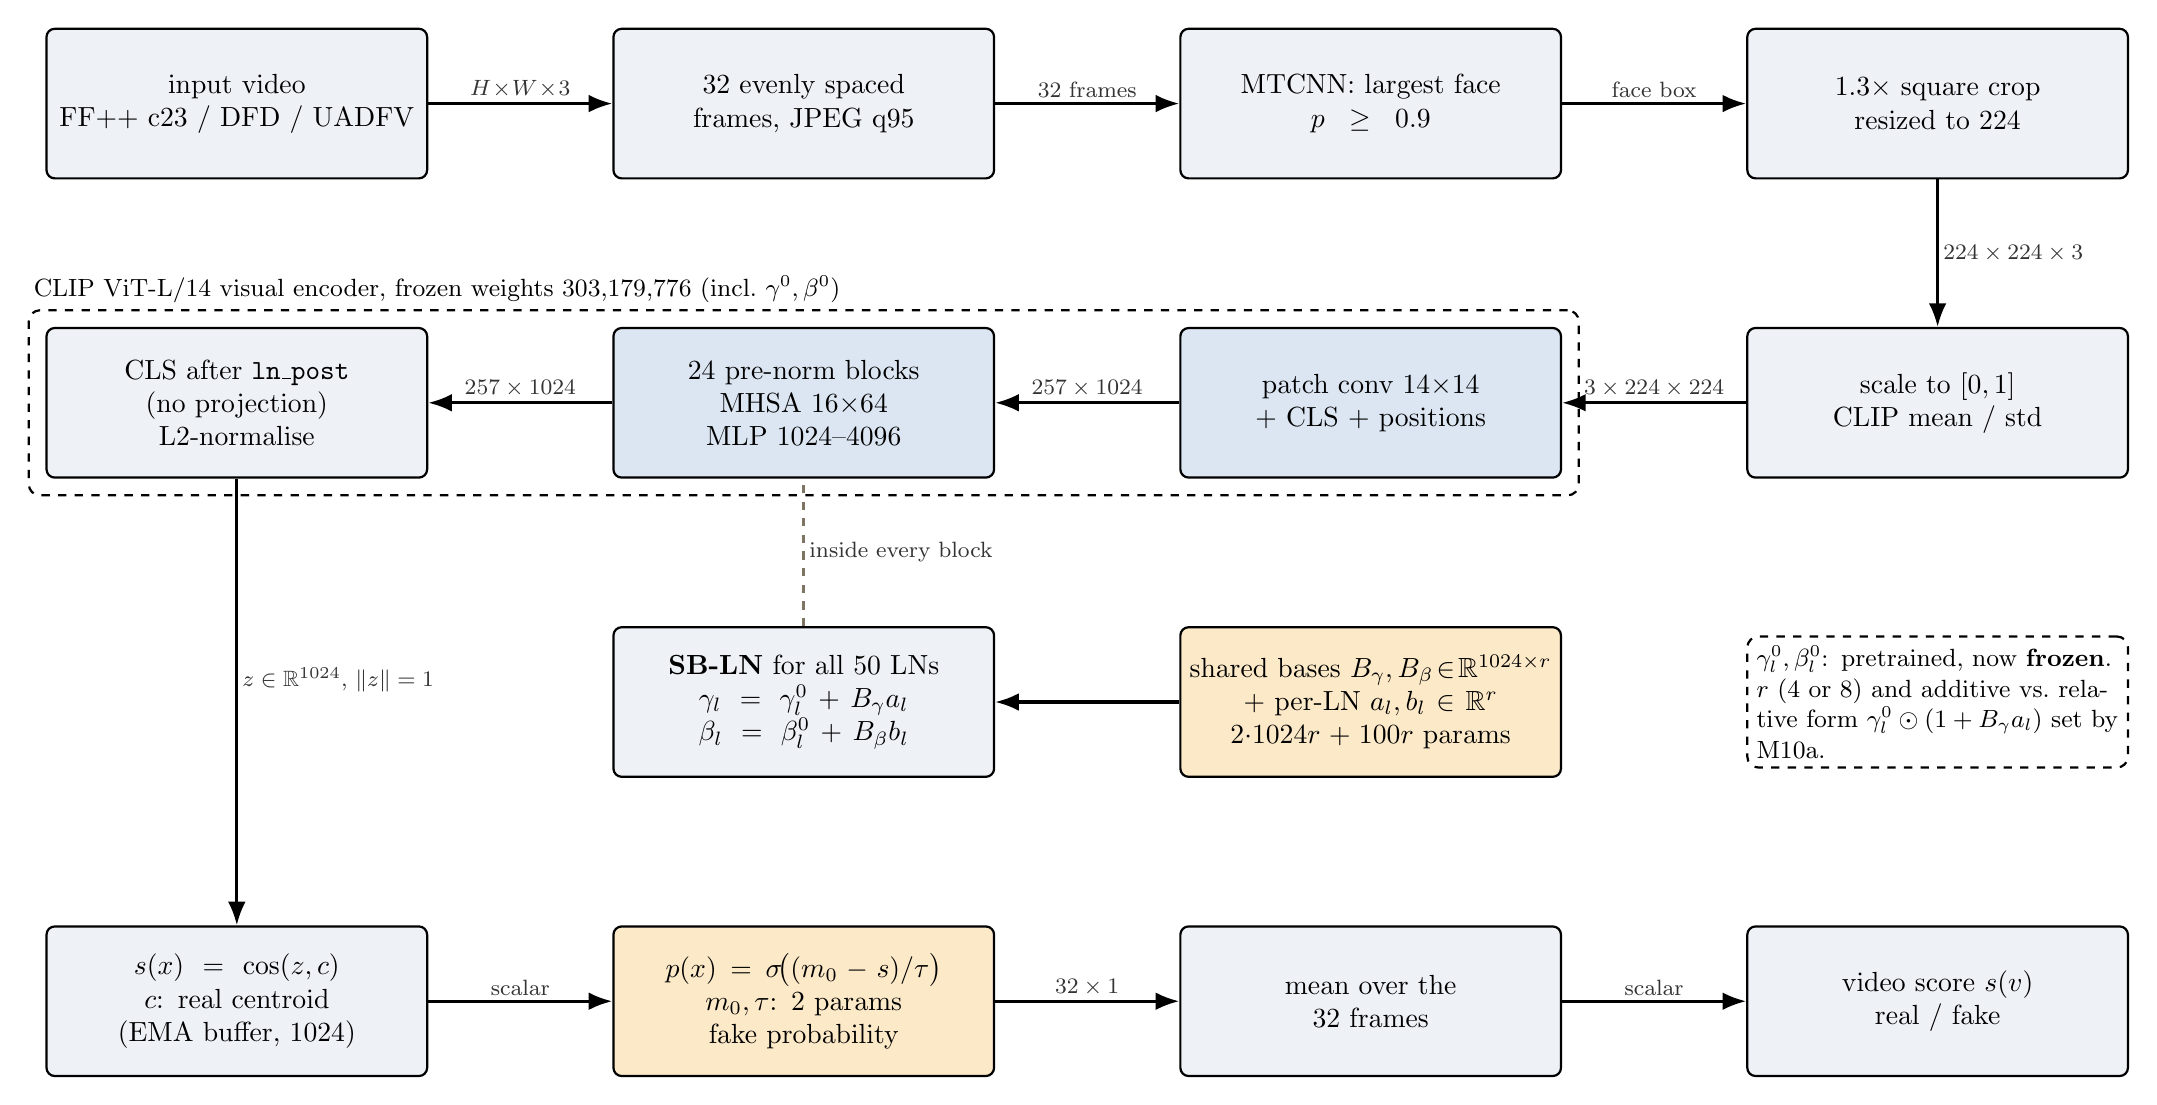
\begin{tikzpicture}[x=72mm,y=-38mm]
% row 1: unchanged preprocessing
\node[blk] (vid) at (0,0) {input video\\FF++ c23 / DFD / UADFV};
\node[blk] (frm) at (1,0) {32 evenly spaced\\frames, JPEG q95};
\node[blk] (det) at (2,0) {MTCNN: largest face\\\(p\ge0.9\)};
\node[blk] (crp) at (3,0) {1.3\(\times\) square crop\\resized to 224};
% row 2: frozen encoder
\node[blk] (pre) at (3,1) {scale to \([0,1]\)\\CLIP mean / std};
\node[frz] (pe)  at (2,1) {patch conv 14\(\times\)14\\+ CLS + positions};
\node[frz] (tr)  at (1,1) {24 pre-norm blocks\\MHSA 16\(\times\)64\\MLP 1024--4096};
\node[blk] (cls) at (0,1) {CLS after \texttt{ln\_post}\\(no projection)\\L2-normalise};
% row 3: SB-LN
\node[blk] (sbln) at (1,2) {\textbf{SB-LN} for all 50 LNs\\\(\gamma_l=\gamma_l^0+B_\gamma a_l\)\\\(\beta_l=\beta_l^0+B_\beta b_l\)};
\node[trn] (sbp)  at (2,2) {shared bases \(B_\gamma,B_\beta\!\in\!\mathbb{R}^{1024\times r}\)\\+ per-LN \(a_l,b_l\!\in\!\mathbb{R}^{r}\)\\\(2{\cdot}1024r+100r\) params};
\node[draw,dashed,rounded corners,font=\small,align=left,text width=46mm,line width=0.8pt] (nt) at (3,2)
 {\(\gamma_l^0,\beta_l^0\): pretrained, now \textbf{frozen}. \(r\) (4 or 8) and additive vs.\ relative form \(\gamma_l^0\odot(1+B_\gamma a_l)\) set by M10a.};
% row 4: real-anchored cosine head
\node[blk] (cos) at (0,3) {\(s(x)=\cos(z,c)\)\\\(c\): real centroid\\(EMA buffer, 1024)};
\node[trn] (hd)  at (1,3) {\(p(x)=\sigma\!\big((m_0-s)/\tau\big)\)\\\(m_0,\tau\): 2 params\\fake probability};
\node[blk] (agg) at (2,3) {mean over the\\32 frames};
\node[blk] (out) at (3,3) {video score \(s(v)\)\\real / fake};
% arrows
\draw[ar] (vid)--node[lab,above]{\(H\!\times\!W\!\times\!3\)}(frm);
\draw[ar] (frm)--node[lab,above]{32 frames}(det);
\draw[ar] (det)--node[lab,above]{face box}(crp);
\draw[ar] (crp)--node[lab,right]{\(224\times224\times3\)}(pre);
\draw[ar] (pre)--node[lab,above]{\(3\times224\times224\)}(pe);
\draw[ar] (pe)--node[lab,above]{\(257\times1024\)}(tr);
\draw[ar] (tr)--node[lab,above]{\(257\times1024\)}(cls);
\draw[ar] (cls)--node[lab,right,pos=0.45]{\(z\in\mathbb{R}^{1024}\), \(\|z\|=1\)}(cos);
\draw[ar] (cos)--node[lab,above]{scalar}(hd);
\draw[ar] (hd)--node[lab,above]{\(32\times1\)}(agg);
\draw[ar] (agg)--node[lab,above]{scalar}(out);
\draw[ar] (sbp)--(sbln);
\draw[line width=1.1pt,dashed,trn!50!black] (sbln)--node[lab,right]{inside every block}(tr);
\begin{scope}[on background layer]
\node[draw,dashed,rounded corners,fit=(pe)(tr)(cls),inner sep=6pt,line width=0.8pt] (bb) {};
\end{scope}
\node[font=\small,anchor=south west,inner sep=2pt] at (bb.north west) {CLIP ViT-L/14 visual encoder, frozen weights 303,179,776 (incl.\ \(\gamma^0,\beta^0\))};
\end{tikzpicture}
\end{center}

\vfill
{\small Replaced from the implemented model: 50 independent LayerNorms (102,400) \(\to\) SB-LN (\(17{,}184\) at \(r=8\), \(8{,}592\) at \(r=4\)); linear head \(1024\to2\) (2,050) \(\to\) real-anchored cosine head (2). Fallback if M10b rejects the cosine head: one-direction head \(p=\sigma(w^\top z+b)\) (1,025). For fixed features the cosine head's frame AUC does not depend on \(m_0,\tau\).}

\newpage
% ---------------------------------------------------------------------
% PAGE 2: SB-LN construction and parameter budget
% ---------------------------------------------------------------------
\begin{center}
{\Large\bfseries Shared-Basis LayerNorm (SB-LN) and Parameter Budget}\\[2pt]
{\small All 50 LayerNorm changes are one \(50\times1024\) matrix of rank \(\le r\); the channel directions are shared, each LayerNorm only chooses \(r\) coefficients.}
\end{center}
\vspace{3mm}

\begin{center}
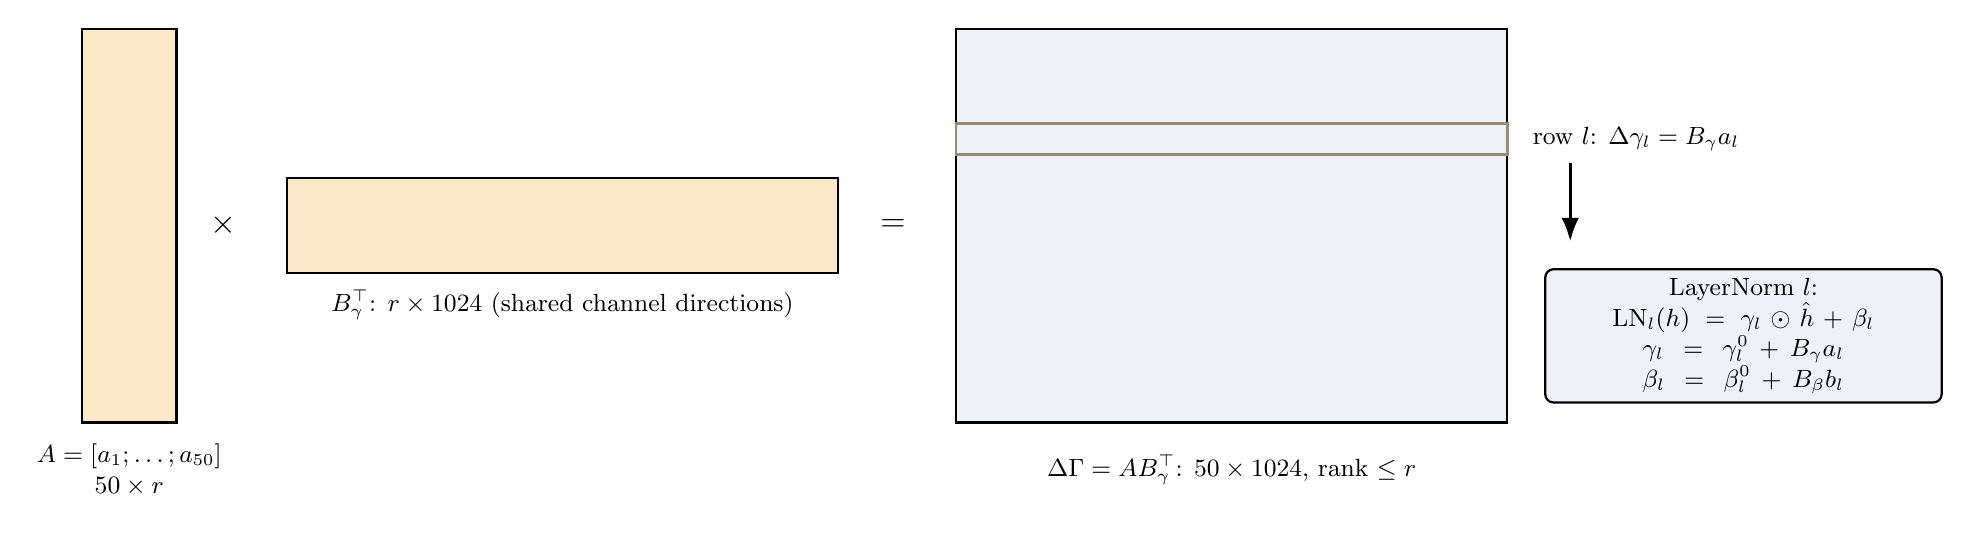
\begin{tikzpicture}[x=1mm,y=1mm]
% coefficient matrix A (50 x r)
\node[draw,fill=trn,minimum width=12mm,minimum height=50mm,line width=0.8pt] (A) at (0,0) {};
\node[font=\small,align=center] at (0,-31) {\(A=[a_1;\dots;a_{50}]\)\\\(50\times r\)};
\node[font=\large] at (12,0) {\(\times\)};
% basis transpose (r x 1024)
\node[draw,fill=trn,minimum width=70mm,minimum height=12mm,line width=0.8pt] (B) at (55,0) {};
\node[font=\small] at (55,-10) {\(B_\gamma^\top\): \(r\times1024\) (shared channel directions)};
\node[font=\large] at (97,0) {\(=\)};
% delta gamma (50 x 1024)
\node[draw,fill=box,minimum width=70mm,minimum height=50mm,line width=0.8pt] (D) at (140,0) {};
\draw[line width=1pt,trn!60!black] (105,9) rectangle (175,13);
\node[font=\small,align=center] at (140,-31) {\(\Delta\Gamma=AB_\gamma^\top\): \(50\times1024\), rank \(\le r\)};
\node[font=\small,anchor=west] at (177,11) {row \(l\): \(\Delta\gamma_l=B_\gamma a_l\)};
\draw[ar] (183,8)--(183,-2);
\node[draw,rounded corners=3pt,fill=box,align=center,font=\small,text width=48mm,line width=0.8pt] at (205,-14)
 {LayerNorm \(l\):\\\(\mathrm{LN}_l(h)=\gamma_l\odot\hat h+\beta_l\)\\\(\gamma_l=\gamma_l^0+B_\gamma a_l\)\\\(\beta_l=\beta_l^0+B_\beta b_l\)};
\end{tikzpicture}
\end{center}
\vspace{2mm}
{\small Same construction for the shift: \(\Delta\mathrm{B}=C B_\beta^\top\), \(C=[b_1;\dots;b_{50}]\). The implemented model is the special case \(r=1024\), \(B=I\) (independent LayerNorms). The private offset of generator \(g\) lives in coefficient space, \((A+\Delta A_g,\;C+\Delta C_g)\), with the bases shared.\par}

\vspace{6mm}
\begin{center}
\small
\begin{tabular}{L{70mm}rrrrrr}
\toprule
model & adapter & head & trainable (deployed) & frozen & total & trainable \% \\
\midrule
implemented GBLA (50 LNs + linear head) & 102,400 & 2,050 & 104,450 & 303,077,376 & 303,181,826 & 0.0345 \\
\textbf{proposed SB-LN \(r=8\) + cosine head} & 17,184 & 2 & \textbf{17,186} & 303,179,776 & 303,196,962 & 0.0057 \\
proposed SB-LN \(r=4\) + cosine head & 8,592 & 2 & 8,594 & 303,179,776 & 303,188,370 & 0.0028 \\
fallback SB-LN \(r=8\) + one-direction head & 17,184 & 1,025 & 18,209 & 303,179,776 & 303,197,985 & 0.0060 \\
\bottomrule
\end{tabular}

\vspace{4mm}
\begin{tabular}{L{70mm}rrr}
\toprule
during training & shared & private (4 generators) & stored \\
\midrule
implemented GBLA (\(\delta_g\) in full \(\theta\) space) & 104,450 & \(4\times104{,}450\) & 522,250 \\
\textbf{proposed, \(r=8\) (\(\delta_g\) in coefficient space)} & 17,186 & \(4\times800\) & \textbf{20,386} \\
proposed, \(r=4\) & 8,594 & \(4\times400\) & 10,194 \\
\bottomrule
\end{tabular}
\end{center}

\vfill
{\small Reduction of deployed trainable numbers: \(6.1\times\) (\(r=8\)), \(12.2\times\) (\(r=4\)); private offsets \(130\times\) smaller per generator at \(r=8\). The real centroid \(c\) is a stored, non-trained buffer of 1,024 numbers (not counted as trainable). Frozen count of the proposed model includes the 102,400 pretrained \(\gamma^0,\beta^0\), which are no longer trained.}

\newpage
% ---------------------------------------------------------------------
% PAGE 3: proposed training workflow
% ---------------------------------------------------------------------
\begin{center}
{\Large\bfseries Proposed Training Workflow --- Coefficient-Space Private Offsets + GBRA Loss}\\[2pt]
{\small GBRA = Generator-Balanced Real-Anchored loss. The weight of each generator is read from the norm of its private offset, which links the private latent space to the loss.}
\end{center}
\vspace{8mm}

\begin{center}
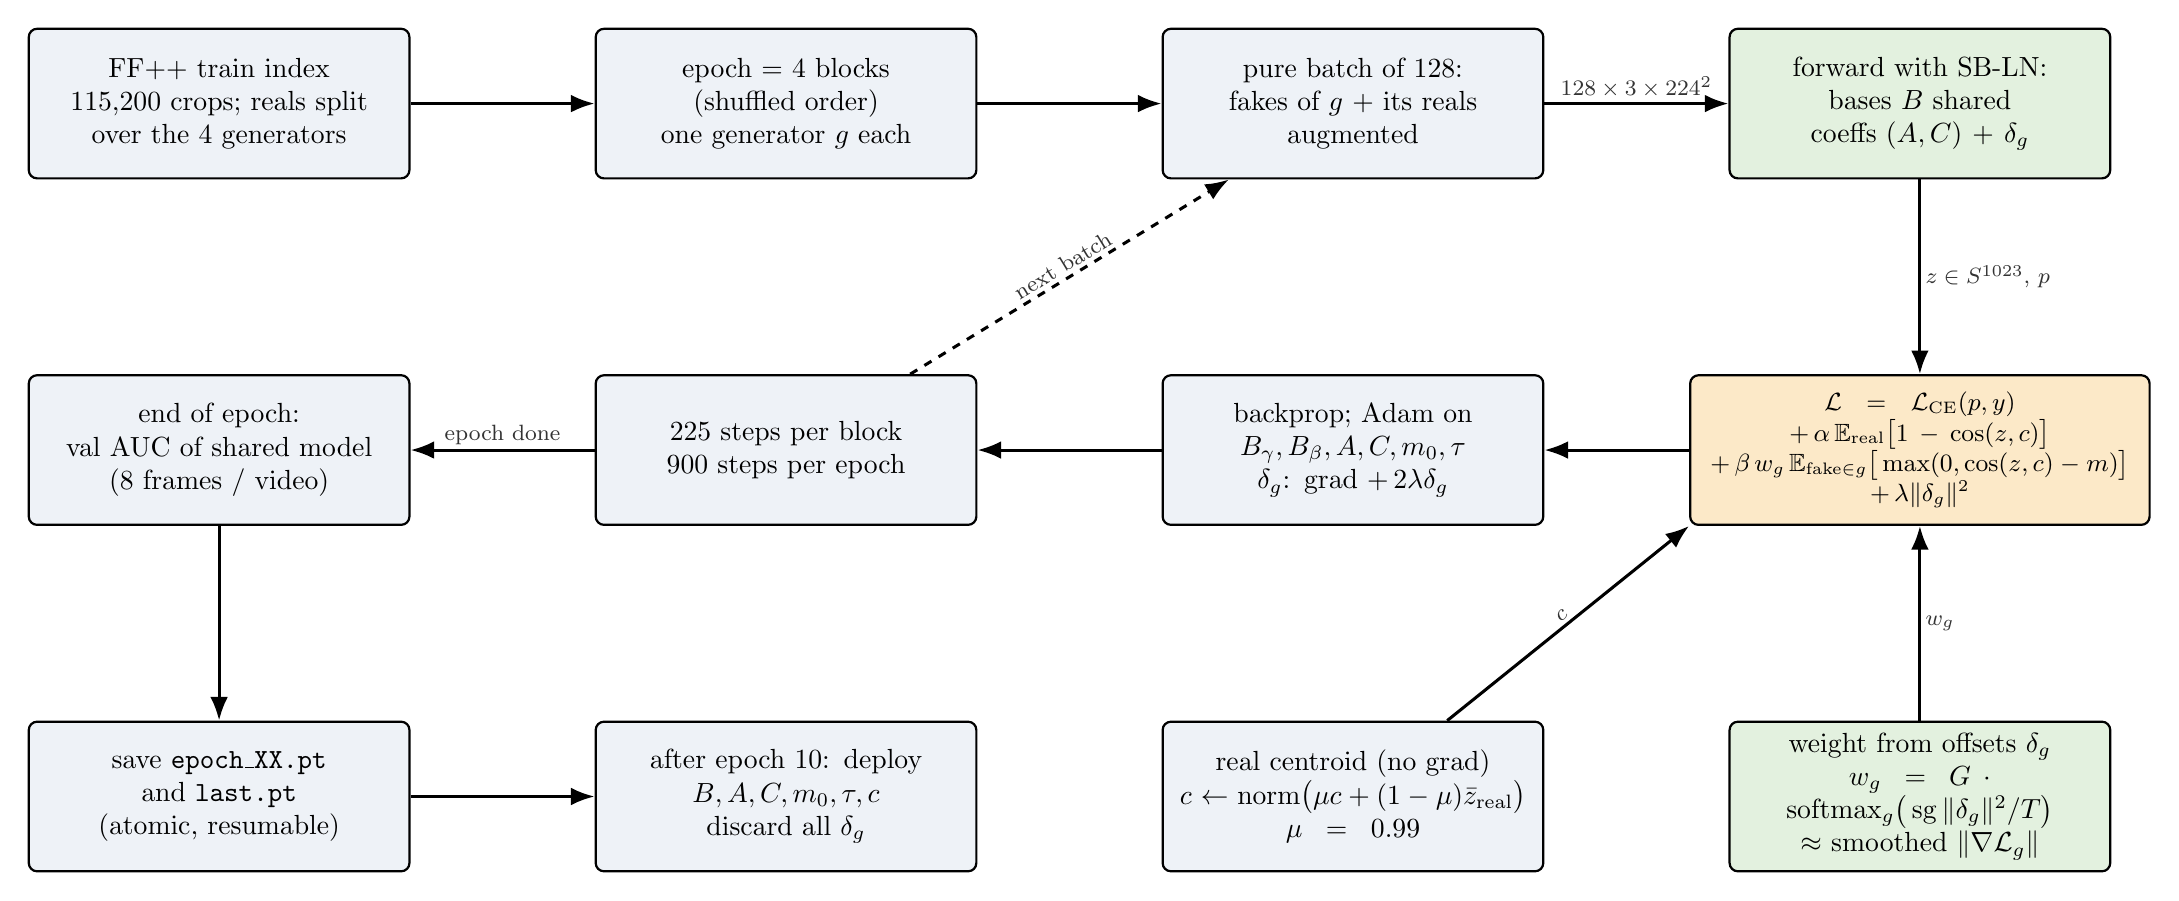
\begin{tikzpicture}[x=72mm,y=-44mm]
\node[blk] (ds)   at (0,0) {FF++ train index\\115,200 crops; reals split\\over the 4 generators};
\node[blk] (blk)  at (1,0) {epoch = 4 blocks\\(shuffled order)\\one generator \(g\) each};
\node[blk] (bat)  at (2,0) {pure batch of 128:\\fakes of \(g\) + its reals\\augmented};
\node[prv] (fw)   at (3,0) {forward with SB-LN:\\bases \(B\) shared\\coeffs \((A,C)+\delta_g\)};
\node[trn,text width=56mm,font=\small] (loss) at (3,1)
 {\(\mathcal{L}=\mathcal{L}_\text{CE}(p,y)\)\\
  \(+\,\alpha\,\mathbb{E}_\text{real}\big[1-\cos(z,c)\big]\)\\
  \(+\,\beta\,w_g\,\mathbb{E}_{\text{fake}\in g}\big[\max(0,\cos(z,c)-m)\big]\)\\
  \(+\,\lambda\|\delta_g\|^2\)};
\node[blk] (bp)   at (2,1) {backprop; Adam on\\\(B_\gamma,B_\beta,A,C,m_0,\tau\)\\\(\delta_g\): grad \(+\,2\lambda\delta_g\)};
\node[blk] (nxt)  at (1,1) {225 steps per block\\900 steps per epoch};
\node[blk] (val)  at (0,1) {end of epoch:\\val AUC of shared model\\(8 frames / video)};
\node[blk] (ck)   at (0,2) {save \texttt{epoch\_XX.pt}\\and \texttt{last.pt}\\(atomic, resumable)};
\node[blk] (fin)  at (1,2) {after epoch 10: deploy\\\(B,A,C,m_0,\tau,c\)\\discard all \(\delta_g\)};
\node[blk] (cent) at (2,2) {real centroid (no grad)\\\(c\leftarrow\mathrm{norm}\big(\mu c+(1-\mu)\bar z_\text{real}\big)\)\\\(\mu=0.99\)};
\node[prv] (wg)   at (3,2) {weight from offsets \(\delta_g\)\\\(w_g=G\cdot\mathrm{softmax}_g\big(\sg\|\delta_g\|^2/T\big)\)\\\(\approx\) smoothed \(\|\nabla\mathcal{L}_g\|\)};
\draw[ar] (ds)--(blk); \draw[ar] (blk)--(bat);
\draw[ar] (bat)--node[lab,above]{\(128\times3\times224^2\)}(fw);
\draw[ar] (fw)--node[lab,right]{\(z\in S^{1023}\), \(p\)}(loss);
\draw[ar] (loss)--(bp); \draw[ar] (bp)--(nxt);
\draw[ar,dashed] (nxt)--node[lab,above,sloped]{next batch}(bat);
\draw[ar] (nxt)--node[lab,above]{epoch done}(val);
\draw[ar] (val)--(ck); \draw[ar] (ck)--(fin);
\draw[ar] (wg)--node[lab,right]{\(w_g\)}(loss);
\draw[ar] (cent)--node[lab,above,sloped]{\(c\)}(loss.south west);

\end{tikzpicture}
\end{center}

\vfill
{\small First-order link: at the optimum of the private objective \(\delta_g\approx-\nabla\mathcal{L}_g(\theta_s)/(2\lambda)\), so \(\|\delta_g\|^2\propto\|\nabla\mathcal{L}_g\|^2\): generators the shared model fits worst (M7b: NeuralTextures) get the largest margin weight, at no extra cost. \(\alpha,\beta,m,T,\lambda,\mu\) are chosen on FF++ validation in M11; nothing is selected on test data. The cosine head's \(c\) and the loss use the same centroid. Planned ablations: \(w_g=1\); loss-based weights (GroupDRO); no private offsets; offsets in full \(\theta\) space; linear vs.\ cosine head; \(r\in\{4,8,16\}\).}

\newpage
% ---------------------------------------------------------------------
% PAGE 4: novelty summary
% ---------------------------------------------------------------------
\begin{center}
{\Large\bfseries Claimed Contributions and Closest Prior Work}\\[2pt]
{\small Based on our literature search (Nov 2026). Claims marked ``pending'' depend on M10a / M10b / M11 results.}
\end{center}
\vspace{3mm}

\small
\renewcommand{\arraystretch}{1.25}
\begin{tabular}{L{8mm}L{56mm}L{82mm}L{68mm}L{30mm}}
\toprule
\# & contribution & what is new & closest prior work & evidence \\
\midrule
N1 & \textbf{Shared-Basis LayerNorm (SB-LN)} & One learned \(r\)-dim channel basis shared by all 50 LayerNorms; each LN learns only \(2r\) coefficients. LN tuning becomes a rank-\(r\) matrix factorisation (\(102{,}400\to2{\cdot}1024r+100r\)). & LN-Tune (AAAI 2024): independent LNs. arXiv 2508.07577: one scalar rescale of LN shifts. ShareLoRA, ASLoRA, RaSA: shared bases for weight matrices, not LN. & M10a (spectrum, truncation) \\
N2 & \textbf{Coefficient-space private latent} & Generator-specific offsets live in SB-LN's coefficient space (\(100r\), 800 per generator at \(r=8\) vs.\ 104,450); bases stay shared, so private and shared models differ only in how they mix common directions. & Our GBLA (full-space offsets); M2/M2b random subspaces failed, this subspace is learned. & M10a \S4; M11 \\
N3 & \textbf{Offset-norm generator weighting} & \(w_g=G\cdot\mathrm{softmax}(\sg\|\delta_g\|^2/T)\): the private offsets act as a free, smoothed per-generator gradient-norm estimate (\(\delta_g\approx-\nabla\mathcal{L}_g/2\lambda\)) that drives the loss. This is the link between the private latent space and the loss. & GroupDRO (ICLR 2020): weights from group loss. TSRL (2026): RL tutor reweighting. DOSS-Weight (speech). None use private-offset norms. & M7b motivation; M11 ablation vs.\ GroupDRO \\
N4 & \textbf{GBRA loss} & Real-anchored compactness plus generator-balanced margins weighted by N3; the same centroid \(c\) is used by the loss and the head, so training and inference match. & Single-Center Loss (CVPR 2021, face forgery): real centre + margin, no generator weighting. OC-Softmax (audio). Centre term credited to them. & M11 \\
N5 & \textbf{Real-anchored cosine head} (pending) & Classifier with 2 trained numbers \(\sigma((m_0-\cos(z,c))/\tau)\), \(c\) a non-trained real centroid; replaces the 2,050-number linear head. & SCL keeps a softmax classifier; OC-Softmax learns the direction. Final check needed before claiming. & M10b \\
N6 & \textbf{Parameter efficiency} & 17,186 deployed (\(6.1\times\) fewer) or 8,594 (\(12.2\times\)); 20,386 stored during training vs.\ 522,250. & LNCLIP-DF / our GBLA: 104,450. & M11 (accuracy at fixed budget) \\
\bottomrule
\end{tabular}

\vfill
{\small Success criteria for M11 (set before training): \(\le\)20k deployed trainable numbers; FaceShifter (unseen) video AUC \(\ge92\); DFD \(\ge96\); held-out NeuralTextures \(\ge64.4\) (the pooled \(\lambda=\infty\) level). Carried over from the implemented work: GBLA shared + private training with only the shared model deployed.}

\end{document}
